\section{Schach Engine}

\subsection{Anforderungen}

% ================================================================================ %
\begin{frame}{Anforderungen}
\begin{itemize}
\item Jede Schach Engine muss bestimmte Anforderungen erfüllen
	\begin{itemize}
		\item Darstellung des Schachbretts
		\item Suche nach den möglichen Spielzügen
		\item Bewertung der Position
	\end{itemize}
\end{itemize}
\end{frame}
% ================================================================================ %

\subsection{Brett Darstellung}

% ================================================================================ %
\begin{frame}{Brett Darstellung}
\begin{itemize}
	\item Brett und Figuren müssen in eine Computer verständliche Form gebracht werden
	\item Eine Möglichkeit der Darstellung sind Bitboards
	\item Jedes Feld wird dargestellt und kann entweder den Wert 0 oder 1 enthalten
	\begin{itemize}
		\item 0 = Keine Figur auf Feld, 1 = Figur auf Feld
	\end{itemize}
	\item Für jeden Figurtyp (6), Figurfarbe (2) und für Rochaden (4) werden Bitboards erstellt
	\begin{itemize}
		\item 16 Bitboards insgesamt
	\end{itemize}
\end{itemize}
\end{frame}



\begin{frame}{Brett Darstellung}
\begin{itemize}
	\item Mögliche Implementierung durch $8 \times 8$ Arrays
	\item Züge können mit Hilfe von logischen Operationen berechnet werden
	\item Vorteil: Können als Input für neuronale Netze verwendet werden können
\end{itemize}
\begin{figure}
\centering
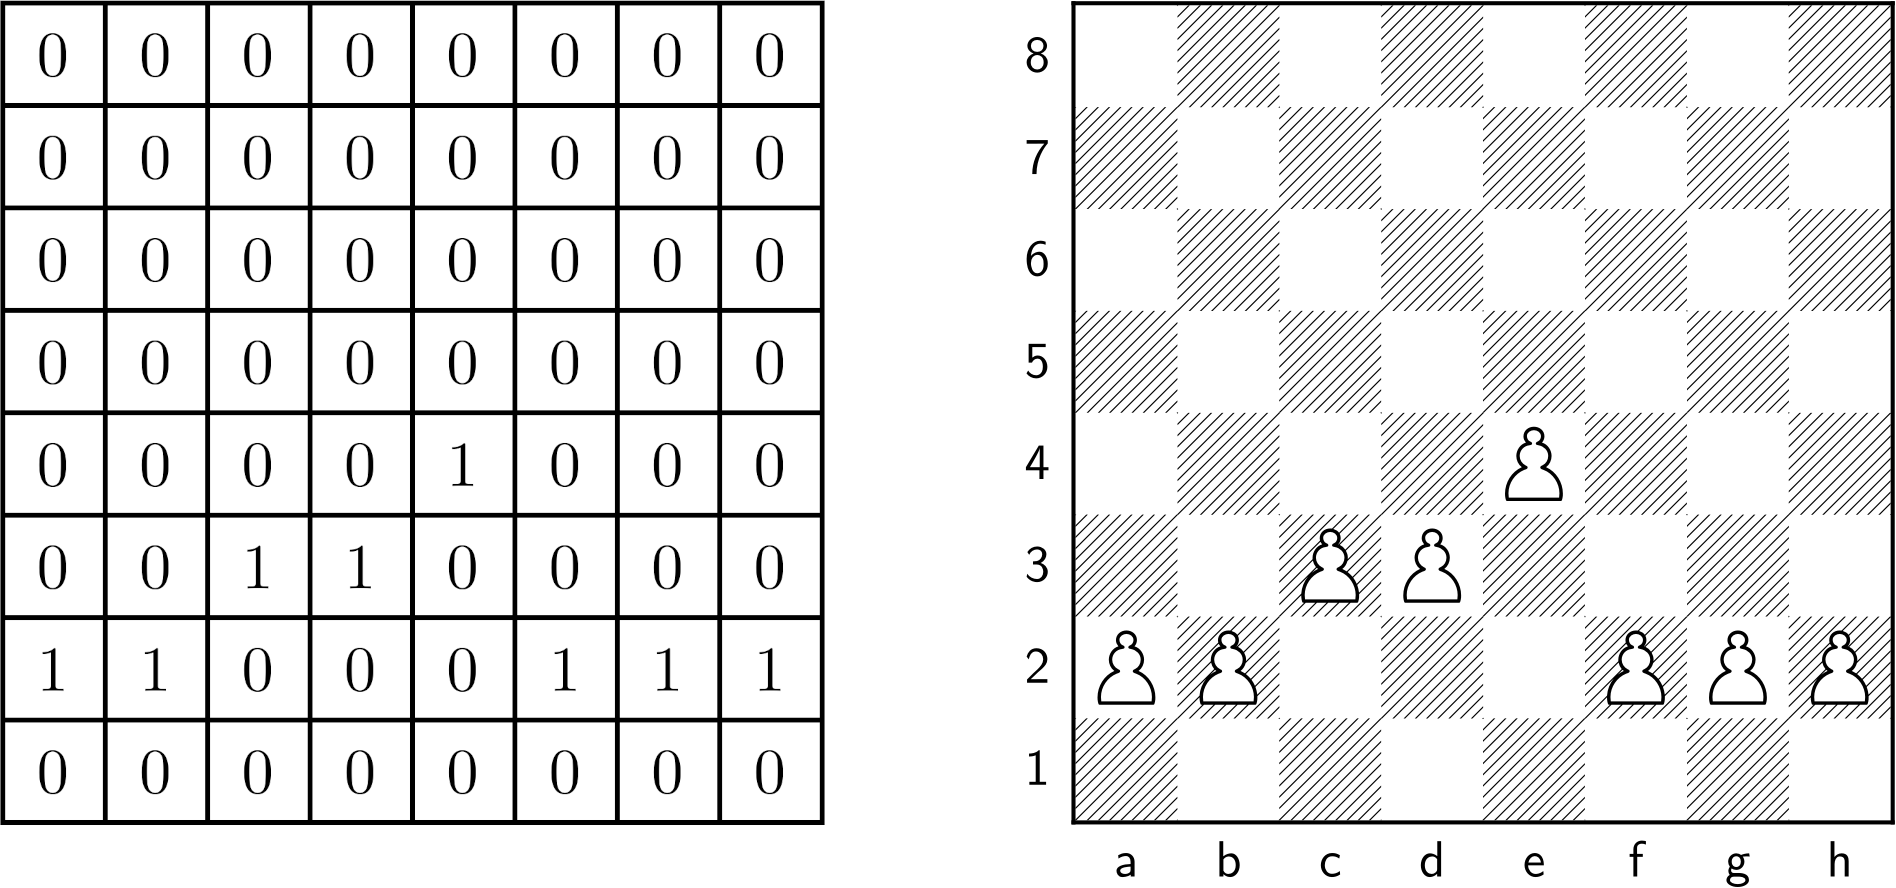
\includegraphics[width=0.45\textwidth]{graphics/bitboard/bitboard_and_chessboard.png}
\end{figure}
\end{frame}
% ================================================================================ %

\subsection{Zugsuche und Positionsbewertung}

% ================================================================================ %
\begin{frame}{Zugsuche und Positionsbewertung}
\begin{itemize}
	\item Schach ist bislang ungelöst
	\item Suche nach dem besten Zug und Bewertung auf der Grundlage von Rechenfertigkeiten und Programmierung
	\item Um den besten Zug zu finden, muss die Engine zwei Aufgaben erfüllen
	\begin{itemize}
		\item Legale, möglichen Züge in aktuellen und folgenden Positionen finden (Zugsuche)
		\item Positionen bewerten
	\end{itemize}
	\item Bekannte Implementierungen: MiniMax/Alpha-Beta Pruning und handgeschriebene Evaluationsfunktion
\end{itemize}
\end{frame}




\begin{frame}{Zugsuche und Positionsbewertung}
\begin{itemize}
	\item Neue Implementierungen: Monte Carlo tree search (MCTS) und Neuronales Netzwerk
	\begin{itemize}
		\item Ansatz mittels maschinellem Lernen
	\end{itemize}
	\item Neuronales Netzwerk zum bewerten einer Position
	\item MCTS zum suchen von Zügen
	\item Pfad mit der besten Gesamtbewertung wird gespielt
\end{itemize}
\end{frame}





\begin{frame}{Zugsuche und Positionsbewertung}
\includegraphics<1>[width=0.9\textwidth]{graphics/alphazero/steps/alphazero_1.png}
\includegraphics<2>[width=0.9\textwidth]{graphics/alphazero/steps/alphazero_2.png}
\includegraphics<3>[width=0.9\textwidth]{graphics/alphazero/steps/alphazero_3.png}
\includegraphics<4>[width=0.9\textwidth]{graphics/alphazero/steps/alphazero_4.png}
\includegraphics<5>[width=0.9\textwidth]{graphics/alphazero/steps/alphazero_5.png}
\end{frame}





\begin{frame}{Zugsuche und Positionsbewertung}
\begin{itemize}
	\item Das Neuronale Netzwerk muss trainiert werden, um eine zuverlässige Ausgabe zu erzeugen
	\item Daten für das Training werden durch Selbstspiel generiert
	\item Zu Beginn existiert ein Programm mit Spielregeln, ein untrainiertes neuronales Netz und der MCTS-Algorithmus
\end{itemize}
\end{frame}




\begin{frame}{Zugsuche und Positionsbewertung}
\begin{enumerate}
	\item Programm spielt gegen sich selbst und zeichnet jedes Spiel auf
	\begin{itemize}
		\item Jede Partie bekommt verloren (-1), unentschieden (0) oder gewonnen (+1) zugerodnet
	\end{itemize}
	\item Neuronales Netzwerk wird geklont und die Parameter werden angepasst
	\item Das neue Programm, spielt gegen das alte Programm
	\item Das Programm, das gewinnt, wird ausgewählt und es beginnt wieder bei 1.
\end{enumerate}
\begin{figure}
\centering
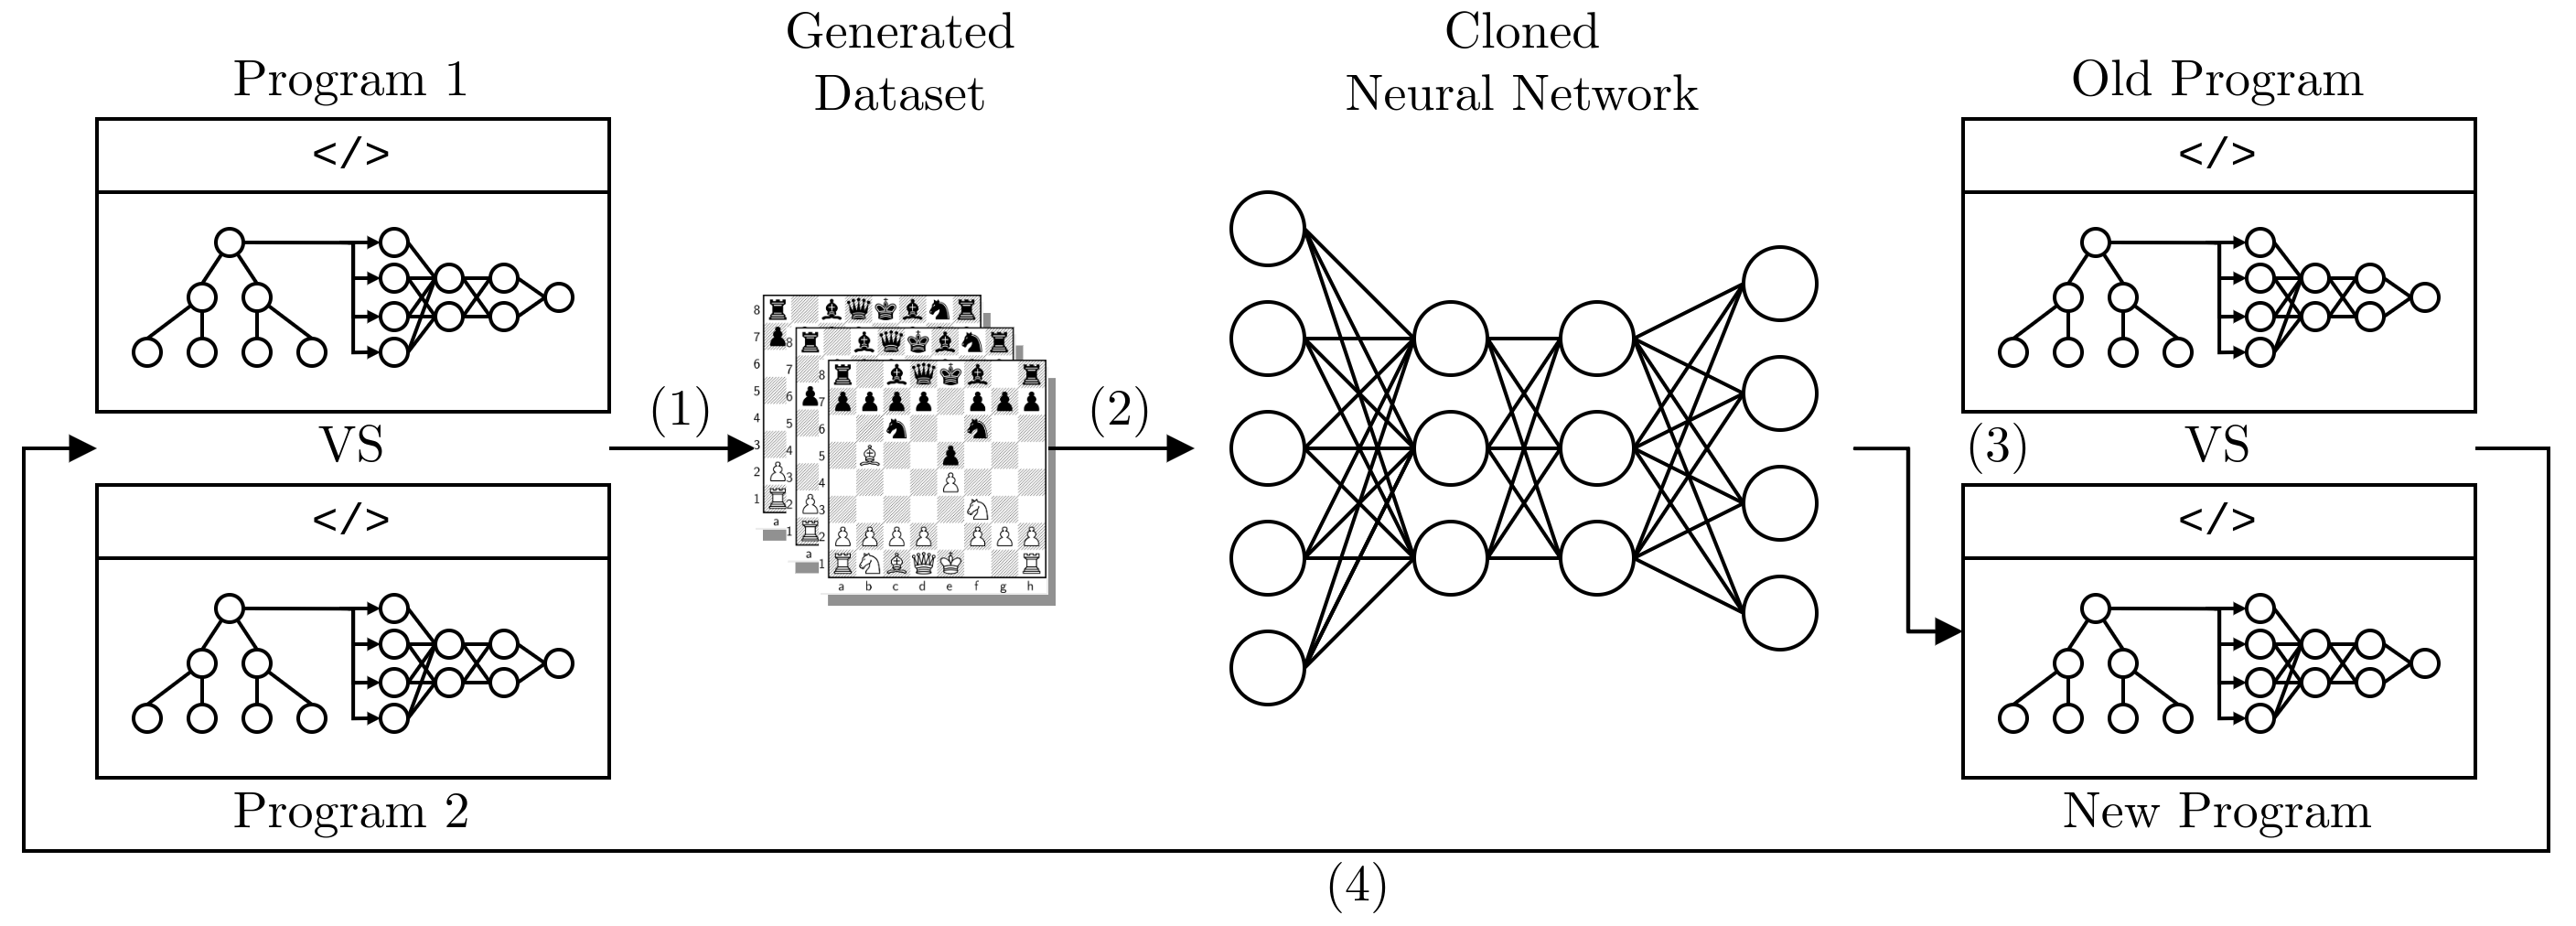
\includegraphics[width=0.7\textwidth]{graphics/alphazero/selfplay.png}
\end{figure}
\end{frame}
% ================================================================================ %

\subsection{Zusammenfassung}

% ================================================================================ %
\begin{frame}{Zusammenfassung}
\begin{itemize}
	\item Von der Schachengine bereitgestellte Informationen:
	\begin{itemize}
		\item Brettdarstellung (Bitboards)
		\item Positionsbewertung ($v$)
		\item Zugwahrscheinlichkeiten ($p$)
		\item Zugpfade
\end{itemize}
\end{itemize}
\end{frame}
% ================================================================================ %